\documentclass{article}

\usepackage{authblk}
\renewcommand\Affilfont{\normalsize}
\usepackage{natbib}
\usepackage{amsmath}
\usepackage{graphicx}

\newcommand{\mbar}{\bar{m}}
\newcommand{\obar}{\bar{o}}
\newcommand{\sumin}{\sum_{i=1}^N}
\newcommand{\bias}{\text{BIAS}}
\newcommand{\rmse}{\text{RMSE}}
\newcommand{\crmse}{\text{CRMSE}}

\title{Normalized Taylor diagrams}
\author[1, 2]{Olivier Gourgue}
\affil[1]{Vrije Universiteit Brussel, Department of Hydrology and Hydraulic Engineering, Pleinlaan 2, 1050 Brussels, Belgium}
\affil[2]{Flanders Hydraulics Research, Flemish Government, Berchemlei 115, 2140 Antwerp, Belgium}

\begin{document}

\maketitle

A Taylor diagram is a polar coordinate plot that summarizes multiple aspects of model performance in a single diagram \citep{Taylor2001}. An even powerful normalized version \citep{Karna2016} is used in this project. This section describes the theoretical aspects behind it.

Let $o_i$ and $m_i$, $i=1, \dots, N$ be observed and modeled time series  of any scalar variable (e.g. water level, velocity component, salinity), respectively. Their mean ($\obar$ and $\mbar$, respectively) and standard deviation ($\sigma_o$ and $\sigma_m$, respectively) are defined as
\begin{eqnarray}
  \obar & = & \frac{1}{N} \sumin o_i, \\
  \mbar & = & \frac{1}{N} \sumin m_i, \\
  \sigma_o^2 & = & \frac{1}{N} \sumin (o_i - \obar)^2, \\
  \sigma_m^2 & = & \frac{1}{N} \sumin (m_i - \mbar)^2.
\end{eqnarray}
The bias (BIAS), root mean square error (RMSE), centered root mean squared error (CRMSE) and correlation coefficient ($R$) are given by
\begin{eqnarray}
  \bias & = & \mbar - \obar, \\
  \rmse^2 & = & \frac{1}{N} \sumin (m_i - o_i)^2, \\
  \crmse^2 & = & \frac{1}{N} \sumin \big((m_i - \mbar) - (o_i - \obar)\big)^2, \\
  R & = & \frac{1}{\sigma_o \sigma_m} \frac{1}{N} \sumin (m_i - \mbar)(o_i - \obar) .
\end{eqnarray}

CRMSE is related to $\sigma_o$, $\sigma_m$ and $R$ as follows \citep{Taylor2001}:
\begin{equation} \label{eq_taylor}
  CRMSE^2 = \sigma_o^2 + \sigma_m^2 - 2 \sigma_o \sigma_m R.
\end{equation}
Making use of the law of cosines, equation (\ref{eq_taylor}) can be visualized in a Taylor diagram \citep{Taylor2001}, a polar coordinate plot where the radial coordinate is the standard deviation and the angular coordinate is $\arccos(R)$. CRMSE then appears as the distance from the position of the observed time series $(\sigma_o, 0)$, as illustrated in Figure \ref{fig_taylor}.

\begin{figure}
  \centering
  \includegraphics[page = 2, width = \textwidth, trim = 13em 10em 11em 51em, clip = true]{figures/Taylor2001.pdf}
  \caption{Taylor diagram where the reference $(\sigma_o, 0)$ and test $\big(\sigma_m, \arccos(R)\big)$ points represent the observed and modeled time series, respectively. Figure by \citet{Taylor2001}.}
  \label{fig_taylor}
\end{figure}

Equation (\ref{eq_taylor}) has the dimension of the considered variable squared. Dividing it by $\sigma_o^2$ leads to dimensionless quantities and the normalized Taylor diagram \citep{Karna2016}:
\begin{equation}
  CRMSE'^2 = 1 + \sigma_m'^2 - 2 \sigma_m' R,
\end{equation}
with
\begin{eqnarray}
  CRMSE' & = & \frac{1}{\sigma_o} CRMSE , \\
  \sigma_m' & = & \frac{\sigma_m}{\sigma_o} .
\end{eqnarray}
In the normalized diagram, the observed time series always lie at $(1, 0)$. 

With Taylor diagrams, one (as in Figure \ref{fig_taylor}) or several model runs are compared to only one reference data set. Indeed, two different observed time series would have different standard deviations and therefore lie on a difference target point $(\sigma_o, 0)$. A different diagram is therefore needed for each available observed time series. It is not the case with normalized Taylor diagrams, as the target point is always $(1, 0)$. Time series at different locations or even from different variables can be displayed on a single diagram (Figure \ref{fig_norm_taylor}).

\begin{figure}
  \centering
  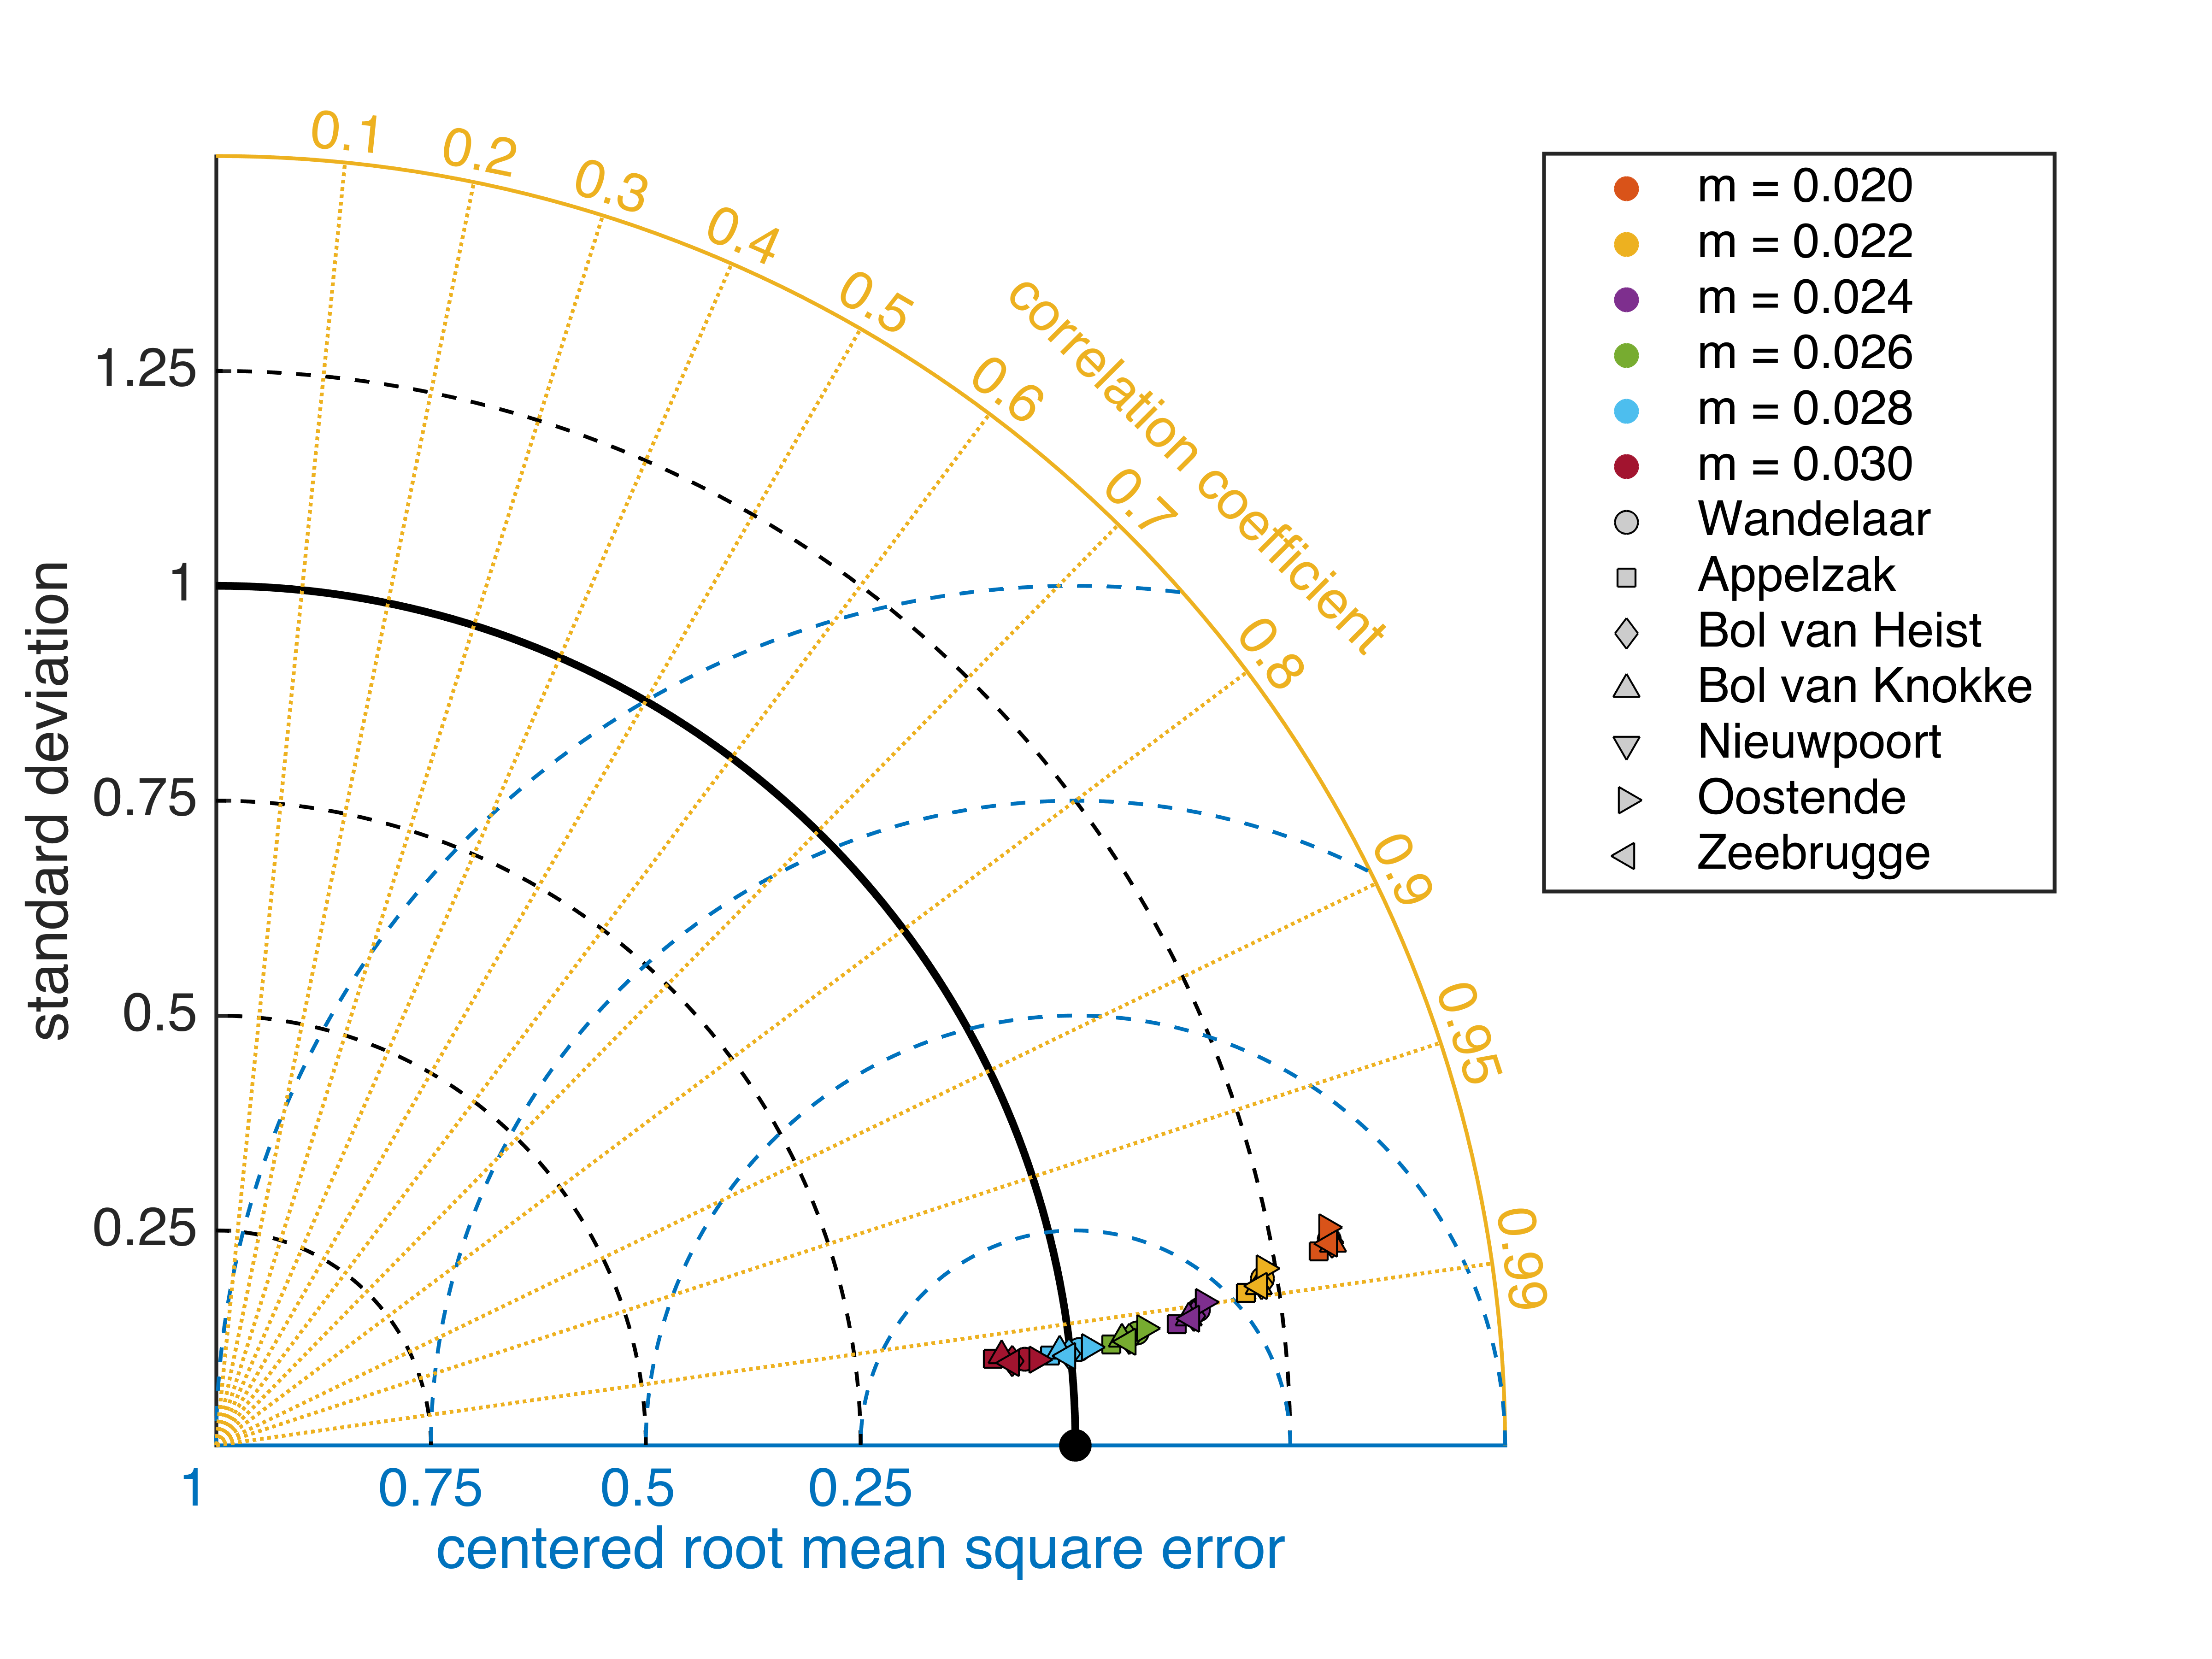
\includegraphics[width = \textwidth]{figures/norm_taylor.png}
  \caption{Normalized Taylor diagrams displaying water elevation time series at different locations of the \textit{Meetnet Vlaamse Banken} (Flemish Banks Monitoring Network), simulated with different values of the Manning coefficient $m$.}
  \label{fig_norm_taylor}
\end{figure}

\bibliography{doc}
\bibliographystyle{apalike}

\end{document}